\section{Rete neurale}
\label{Rete neurale}

La libreria utilizzata per sviluppare la Rete neurale \`e stata \textit{ConvNetJS}. L'aspetto positivo di tale scelta \`e stata la semplicit\`a nell'utilizzo del linguaggio javascript; l'aspetto negativo ha riguardato la totale mancanza di mantenibilit\`a della libreria stessa che comporta la scarsit\`a di esempi applicativi, oltre alla documentazione ufficiale, che costringono lo sviluppatore ad una ricerca approfondita personale in un ambiente ove lo nozioni si presentano scarse e a continue prove per verificare la validit\`a del codice prodotto.
\begin{figure}[H]
\centering
	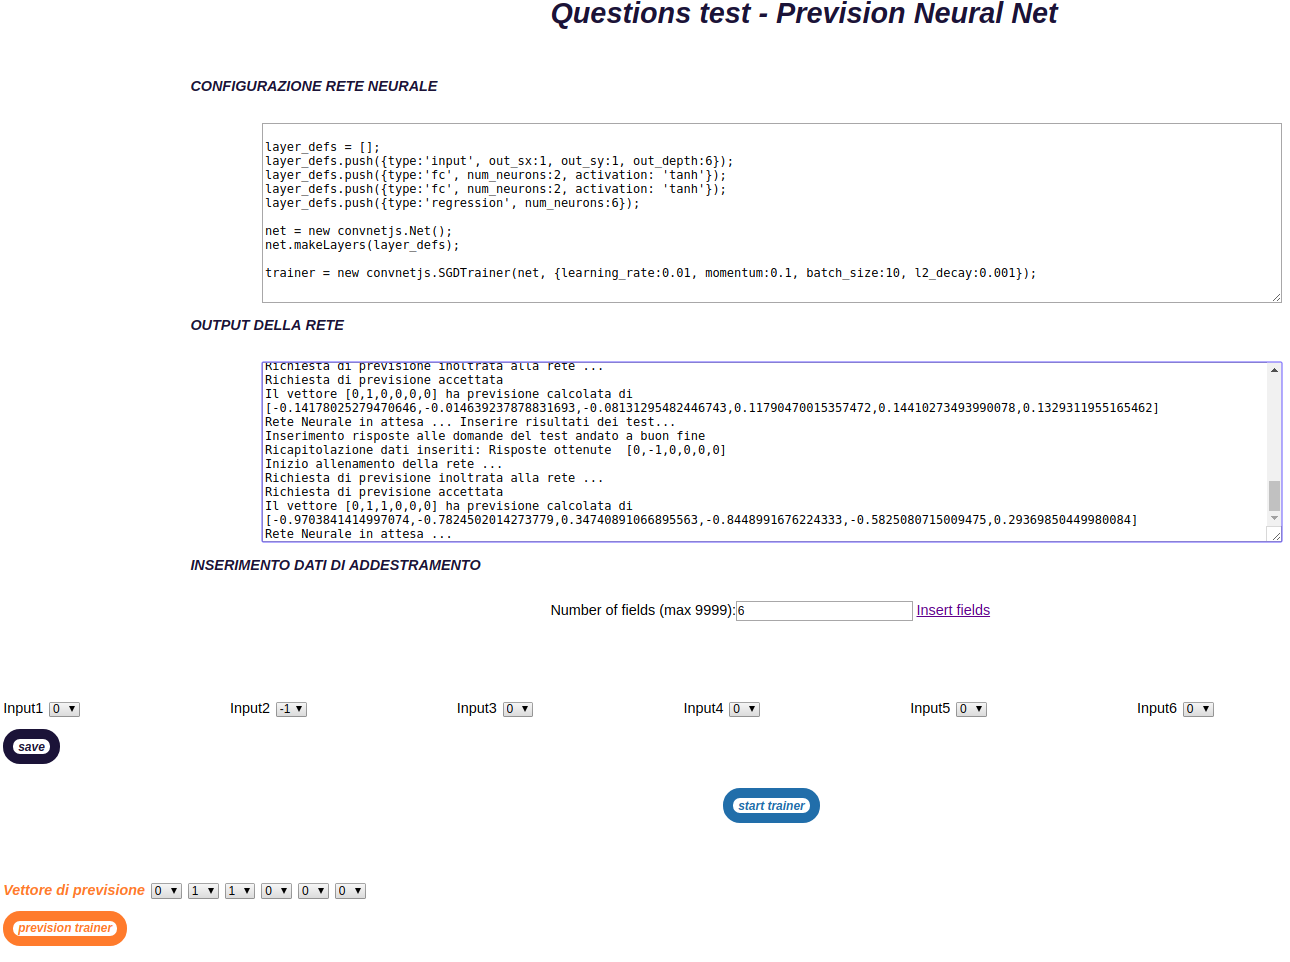
\includegraphics[width=1\linewidth]{./image/GUI-rete-neurale.png}
	\caption{Interfaccia utente della Rete neurale di prova.}
\end{figure}
\noindent
Durante il periodo 24/05 - 31/05 mi sono occupata dello sviluppo di una Rete neurale in grado di ricevere in input un training set di dimensione 6 e di restituire una previsione sui dati di apprendimento ricevuti.
\noindent
Il problema che la rete mira ad analizzare \`e quello discusso nel precedente capitolo \textit{Analisi dei dati di probabilit\`a}
\\\\
Per aggevolare l'apprendimento della rete, ed ottenere delle previsioni stabili mi sono occupata di implementare due metodi di generazione randomica di dati in modo da far apprendere massiciamente la stessa.
Il dato prodotto consiste in un vettore di 6 elementi, composto da  -1, 0 e 1 con il seguente criterio:
\begin{itemize}
\item \textbf{-1}: la domanda x non \`e stata posta al candidato;
\item \textbf{0}: la domanda x \`e stata posta al candidato che ha risposto in maniera errata;
\item \textbf{1}: la domanda x \`e stata posta al candidato che ha saputo rispondere correttamente.
\end{itemize}
\noindent
Il primo metodo che ho sviluppato si occupa di generare un vettore di dati di apprendimento basandosi esclusivamente su come le domande sono interconnesse tra di loro (grazie all'uso di un grafo della conoscenza costruito ad hoc); il secondo metodo ripropone quanto perseguito dal primo metodo con il valore aggiunto di generazione di un profilo randomico di un candidato, che tiene conto della  probabilit\`a di risposta ad una domande seguendo la formula P(A)= $\frac{1}{3}+\frac{1}{6}P(S_1)+\frac{2}{3}P(S_2)$.

\subsection{Test effettuati}
\label{Test effettuati}

Alcune decisioni che ho preso durante la configurazione della rete riguardano i seguenti settori:
\begin{enumerate}
\item Una rete neurale non deve, per fornire dei dati attendibili, possedere un numero di neuroni troppo elevato rispetto al trainset effettuato; altrimenti la previsione  ritornerebbe l'identit\`a del vettore di input della stessa, come conseguenza diretta della capacit\`a troppo elevata di immagazzinare dati.
\item I layers, ho deciso, di allenarli mediante tecnica di regressione, che permette l'inserimento in input di una funzione obiettivo e l'ottenimento di un risultato, in output, anche in virgola mobile e composto di tanti elementi quanti sono i neuroni di regressione dichiarati. Per la mia rete di prova \`e necessario dichiarare  6 neuroni in regressione perch\`e l'output, appunto, che ci si aspetta dal sistema \`e di 6 elementi.
\item Per costruire un dataset di dati consistente che permettesse alla rete di imparare qualcosa ho costruito un grafo della conoscenza con lo scopo di mettere in relazione degli argomenti che coinvolgono uno o pi\`u domande.
\begin{figure}[H]
\centering
	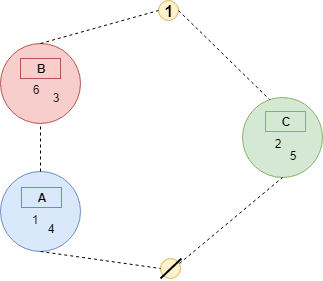
\includegraphics[width=0.60\linewidth]{./image/grafo_trainset.png}
	\caption{Grafo rappresentante le relazioni esistenti tra il set di domande di prova.}
\end{figure}
\noindent
Per svolgere l'apprendimento ogni vettore, facente parte del dataset, viene dato in pasto alla rete che a sua volta provvede alla sua assimilazione come conoscenza mediante la tecnica dell'autoencoder, ovvero la rete impara il vettore riducendone lo spazio occupato.
\item Per creare il dataset ho ritenuto sufficiente generare \textit{2000} vettori di risposta in modo da compiere in maniera esaustivo l'apprendimento della rete.
\end{enumerate}
\noindent
Il vettore passato in input per svolgere le previsioni \`e \textit{[0,1,0,0,0,0]}\\
\noindent. 
Di seguito riporto quanto \`e stato rilevato in fase di test.

\subsubsection{Configurazione della rete: 4 neuroni per ciascuno dei 2 layers}
\label{Configurazione della rete: 4 neuroni per ciascuno dei 2 layers}

Configurazione della rete utilizzata:\\
\begin{verbatim}layer_defs = [];
layer_defs.push({type:'input', out_sx:1, out_sy:1, out_depth:6});
layer_defs.push({type:'fc', num_neurons:4, activation: 'tanh'});
layer_defs.push({type:'fc', num_neurons:4, activation: 'tanh'});
layer_defs.push({type:'regression', num_neurons:6});

net = new convnetjs.Net();
net.makeLayers(layer_defs);

trainer = new convnetjs.SGDTrainer(net, {learning_rate:0.01,
 momentum:0.1, batch_size:10, l2_decay:0.001});
\end{verbatim}
\noindent
I layers utilizzati sono 2 e compositi da 4 neuroni.

\paragraph{Training set standard a 4 neuroni per ciascuno dei 2 layers}\mbox{}
\label{Training set standard a 4 neuroni per ciascuno dei 2 layers}
\\
\noindent
\begin{itemize}
\item \begin{verbatim}[0.18394862760524544,0.5427447874383465,0.4475798470511032,
-0.2002756172921305,0.07023832331402126,-0.38412626496750873] \end{verbatim}
Appaiono in relazione le domande 1, 2, 3, 5 e 4, 6.\\
Gli scostamenti tra le coppie 2 e 5 sono consistenti con quelle che sono le relazioni  di dipendenza fra le domande; invece per quanto concerne le coppie 2, 5 e 1, 4 vi \`e una differenza che va dallo 0.3 allo 0.5 circa; che mi sembra troppo per venire associata solamente alla presenza di valori -1 all'interno del vettore di training. Anche la valutazione del valore 1 nel vettore di previsione non mi sembra una motivazione sufficiente.
Le domande 3 e 6 si dovrebbero presentare con una positivit\`a inferiore rispetto a 1 e 4; nel test in analisi questo vale per la domanda 1 e 4 in relazione con la domanda 6, negli altri casi non si \`e conformi a tale regola.

\item \begin{verbatim}[-0.11235743604300916,-0.39879459369010783,-0.6219582601088702,
0.22754749414916,-0.3307584554090044,-0.39007701490038627] \end{verbatim}\\
Appaiono in relazione le domande 1, 2, 3, 5, 6 e 4.\\
Gli scostamenti tra le coppie 3 e 6, 2 e 5 sono consistenti con quelle che sono le relazioni di dipendenza fra le domande; invece per quanto concerne la coppia 1 e 4 vi \`e una differenza minima dello 0.2, dovuta dalla presenza di -1  all'interno dei vettori di training.
Le domande 3 e 6 si dovrebbero presentare con una positivit\`a inferiore rispetto a 1 e 4; nel test in analisi sia la domanda 1 che 4 si presentano conformi alla regola.

\item \begin{verbatim}[-0.2399988601091234,0.09747007794669733,0.5093732175811206,
0.06546467766710193,0.05567129781511258,-0.11672474718649554]\end{verbatim}\\
Appaiono in relazione le domande 1, 4, 6 e 2, 3, 5.\\
Gli scostamenti tra le  coppie 1, 4 e 2, 5 sono consistenti con quelle che sono le relazioni di dipendenza fra le domande, invece per quanto concerne le coppia 3, 6 vi \`e una differenza che supera lo 0.5; che mi sembra troppo per venire associata solamente alla presenza di valori -1 all'interno del vettore di training.
Le domande 3 e 6 si dovrebbero presentare con una positivit\`a inferiore rispetto a 1 e 4; nel test in analisi solo la domanda 4 in confronto con la domanda 6 rispetta la regola.

\item \begin{verbatim}[0.21422605841447054,-0.2636944179712092,-0.3706563171790509
,0.7764017490883244,-0.23816083562639187,-0.2524885890953481]\end{verbatim}
Appaiono in relazione 1, 4 e 2, 3, 5, 6.\\
Gli scostamenti tra le coppie  1  e 4, 2 e 5, 3 e 6 sono consistenti con quelle che sono le relazioni di dipendenza fra le domande.
Le domande 3 e 6 si dovrebbero presentare con una positivit\`a inferiore rispetto a 1 e 4; nel test in analisi tale regola viene rispettata perfettamente
\end{itemize}


\paragraph{Training set con generazione del profilo di un candidato e calcolo delle probabilit\`a di risposta a 4 neuroni per ciascuno dei 2 layers}\mbox{}
\label{Training set con generazione del profilo di un candidato e calcolo delle probabilita di risposta a 4 neuroni per ciascuno dei 2 layers}
\\
\noindent
\begin{itemize}
\item  \begin{verbatim}[-0.2231017609955856,-0.16052488782458485,-0.019367797676560772,
0.44513277709765614,0.31332777238518317,0.18420998695814583]
\end{verbatim}
Appaiono in relazione le domande 1, 2, 3 e 4, 5, 6.\\
Le coppie 1 e 4, 3 e 6, 2 e 5 non sono pi\`u in relazione stretta con una differenza che va dallo 0.1 allo 0.5 circa. La domanda 1 presenta una positivit\`a inferiore rispetto alla domanda sia 3 che 6 non mostrandosi cos\`i conforme alla regola per una differenza attorno allo 0.3 - 0.5, invece la domanda 4 risulta conforme. L'anomalia pu\`o venire ricondotta all'uso di un set con dati "spuri", calcolati mediante la probabilit\`a che un candidato ha di rispondere correttamente o meno ad una i-esima domanda (tale formula ha fatto venire meno la validit\`a parziale delle relazioni che intercorrono tra le domande) che alla presenza dei valori -1 del vettore di training. Il secondo fattore per\`o ha sicuramente un influenza inferiore rispetto al primo sui risultati ottenuti.

\item \begin{verbatim}[0.14156677163032302,-0.463390621754713,-0.005961372184182835,
0.4296214536241051,-0.14928047861127153,0.07826607623462487]
\end{verbatim}
Appaiono in relazione le domande 1, 4, 6 e 2, 3, 5.\\
La coppia 3 e 6 non \`e pi\`u in relazione stretta ma con una differenza dello 0.07; questo non vale per le coppie 2, 5 e 1, 4 che rimangono conformi alla regola. Sia le domanda 4 che 1 si mostrano con una positivit\`a superiore rispetto alla domanda 3 e 6 presentandosi conforme alla regola.

\item  \begin{verbatim}[0.33370457154838096,0.6819324925536909,0.0677395998504201,
-0.5223246783586419,0.14296539819732018,1.2255342565068268]
\end{verbatim}
Appaiono in relazione le domande 1, 2, 3, 5 e  4, 6.\\
Le domanda 1 e 4, 3 e 6 non sono pi\`u in relazione stretta ma con una differenza importante che oscilla tra lo 0.8 e 1.22 circa. La domanda 1 presenta una positivit\`a inferiore rispetto alla domanda alla 3 ma non rispetto alla domanda 6, mostrandosi cos\`i parzialmente conforme alla regola per una differenza dello 0.9 circa. Lo stesso vale per la domanda 4. L'anomalia pu\`o venire ricondotta all'uso di un set con dati "spuri"  usati per effettuare il training degli stessi.

\item  \begin{verbatim}[0.2794050630320866,0.06927124508771161,0.4651627304680603,
0.08783394507854103,0.07418275088665362,-0.3096950751976722]\end{verbatim}
Appaiono in relazione le domande 1, 2, 3, 4, 5  e 6 (a parte).\\
Le domanda 1 ,4 e 2, 5  sono in relazione stretta, questo non vale per la coppia 3, 6 che ha una differenza circa dello 0.7. La domanda 4 presenta una positivit\`a superiore rispetto alla domanda sia 3 che 6 presentandosi conforme alla regola; invece la domanda 1 risulta conforme solo nel rapporto con la domanda 6 ove \`e una differenza dello 0.6 circa. L'anomalia pu\`o venire ricondotta all'uso di un set con dati "spuri" usati per il effettuare il training degli stessi.
\end{itemize}

\paragraph{Osservazioni}\mbox{}
\label{Osservazioni su rete a 4 neuroni per ciascuno dei 2 layers}
\\\\
\noindent
La configurazione testata si compone di 4 neuroni a layer su una base di 2000 test correndo il rischio di avere una rete che apprende troppo e come effetto negativo "veda" addirittura cose che non esistono.\\
Per fare un 'ulteriore verifica del sistema da me sviluppato ne ho mutato la configurazione riducendo il numero di neuroni presenti in ciascun layers e/o il numero di layers presenti.\\
Le nuove configurazione su cui ho effettuato i test sono esposte nei paragrafi seguenti.

\subsubsection{Configurazione della rete a 2 neuroni per ciascuno dei 2 layers}
\label{Configurazione della rete a 2 neuroni per ciascuno dei 2 layers}
Configurazione della rete utilizzata:\\
\begin{verbatim}layer_defs = [];
layer_defs.push({type:'input', out_sx:1, out_sy:1, out_depth:6});
layer_defs.push({type:'fc', num_neurons:2, activation: 'tanh'});
layer_defs.push({type:'fc', num_neurons:2, activation: 'tanh'});
layer_defs.push({type:'regression', num_neurons:6});

net = new convnetjs.Net();
net.makeLayers(layer_defs);

trainer = new convnetjs.SGDTrainer(net, {learning_rate:0.01,
 momentum:0.1, batch_size:10, l2_decay:0.001});
\end{verbatim}
\noindent
I layers utilizzati sono 2 compositi da 2 neuroni.

\paragraph{Training set standard su rete a 2 neuroni per ciascuno dei 2 layers}\mbox{}
\label{Training set standard su rete a 2 neuroni per ciascuno dei 2 layers}
\\
\noindent
\begin{itemize}
\item \begin{verbatim}[1.156980429249762,0.06806851158038928,0.3113362862886465,
0.17218787779201644,0.34650990282652194,-0.8215874801856704]\end{verbatim}
Appaiono in relazione le domande 1, 2, 3, 4  e 6 a parte.\\
Gli scostamenti tra le coppie  1 e 4, 2 e 5 sono consistenti con quelle che sono le relazioni di dipendenza fra le domande; invece per la coppia 3 e 6 i segni si presentano opposti con una differenza pesante che supera 1.
Le domande 3 e 6 si dovrebbero presentare con una positivit\`a inferiore rispetto a 1 e 4, la regola viene rispettata nel caso della domanda 1 che supera di netto la frequenza di 3 e 6; poco male per la domanda 4 che supera esclusivamente la domanda 6 ma la differenza con la frequenza della domanda 1 sta nell'ordine di centesimi da poter associare ad alterazioni dovute alla presenza di valori -1 nel vettore di training.

\item \begin{verbatim}[0.04982696367584444,0.11290459035591142,-0.0696298921764785, 
0.18228607258850865,0.49713850861314235,-0.012948163156710699]\end{verbatim}
Appaiono in relazione le domande 1, 2, 4, 5 e 3, 6.\\
Gli scostamenti tra le coppie 1, 4 e 2, 5  e 3, 6 sono consistenti con quelle che sono le relazioni di dipendenza fra le domande.
Le domande 3 e 6 si dovrebbero presentare con una positivit\`a inferiore rispetto a 1 e 4, la regola viene rispettata sia dalla domanda 6 che 3.

\item \begin{verbatim}[0.19504797225824305,-0.2295101910352556,-0.028760245350834636,
0.007144898117011814,-0.056011983451495176,-0.1803934455401963]\end{verbatim}
Appaiono in relazione le domande 1, 4 e 2, 3, 5, 6.\\
Gli scostamenti tra le coppie 1, 4 e 2, 5 e 3, 6 sono consistenti con quelle che sono le relazioni di dipendenza fra le domande
Le domande 3 e 6 si dovrebbero presentare con una positivit\`a inferiore rispetto a 1 e 4, la regola viene rispettata pienamente sia dalla domanda 3 che 6.

\item \begin{verbatim}[0.08339384459022353,-0.15782370764467343,0.0005080967853213457,
-0.020723132326211795,-0.03207289911077578,0.004139946640153436]
\end{verbatim}
Appaiono in relazione le domande 1, 3, 6 e 2, 4, 5.\\
Gli scostamenti tra le coppie 3, 6 e 2, 5 sono consistenti con quelle che sono le relazioni di dipendenza fra le domande; invece per la coppia 1 e 4 i segni sono opposti con una differenza trascurabile che posso far ricondurre la alla presenza dei valori -1 nel vettore di training essendo che la differenza di valore \`e inferiore allo 0.18.
Le domande 3 e 6 si dovrebbero presentare con una positivit\`a inferiore rispetto a 1 e 4, la regola viene non rispettata dalla domanda 6 nei confronti della domanda 4  e dalla domanda 3 nei confronti con la domanda 4; ma in ogni caso la differenza \`e marginale  e posso sempre ricondurla ad oscillazioni della rete.
\end{itemize}


\paragraph{Training set con generazione del profilo di un candidato e calcolo delle probabilit\`a di risposta a 2 neuroni per ciascuno dei 2 layers}\mbox{}
\label{Training set con generazione del profilo di un candidato e calcolo delle probabilita di risposta a 2 neuroni per ciascuno dei 2 layers}
\\
\noindent
\begin{itemize}
\item  \begin{verbatim}[0.2594500646454124,0.7539496003736311,-0.09465357747231457,
-0.4505658641560928,0.6243547972902108,0.20289597452949498]\end{verbatim}
Appaiono in relazione le domande 1, 6, 2, 5 e 3, 4 (a parte).\\
Le domande 3, 6 e 1, 4 non sono pi\`u in relazione stretta con per\`o una differenza minima dello 0.11 circa e dello 0.6; invece la coppia 2, 5 rimane consistente. La domanda 1 presenta una positivit\`a superiore rispetto alla domanda sia 3 che 6 presentandosi conformi alla regola; invece la domanda 4 risulta non conforme nei confronti della domanda 6 per un valore attorno allo 0.5 - 0.6. L'anomalia pu\`o venire ricondotta all'uso di un set con dati "spuri", calcolati mediante la probabilit\`a che un candidato ha di rispondere correttamente o meno ad una i-esima domanda (tale formula ha fatto venire meno la validit\`a parziale delle relazioni che intercorrono tra le domande) che alla presenza dei valori -1 del vettore di training. Il secondo fattore per\`o ha sicuramente un influenza inferiore rispetto al primo sui risultati ottenuti.

\item  \begin{verbatim}[0.07034384333187345,-0.14013991734362666,0.10735038538055158,
0.021294102956278014,-0.09810179582025243,-0.044724358939888444]\end{verbatim}
Appaiono in relazione le domande 1, 3, 4 e 2, 5, 6.\\
La coppia 3, 6 non \`e pi\`u in relazione stretta per\`o con una differenza trascurabile dello 0.1 circa; le coppie 2, 5 e 1, 4 rimangono invece consistenti. Le domande 1 e 4 si mostrano con una positivit\`a inferiore rispetto alla domanda 3 in relazione con la 1 non presentandosi conforme alla regola per una differenza dello 0.03 circa. La regola, invece viene rispettata per tutti gli altri casi. L'anomalia pu\`o venire ricondotta all'uso di un set con dati "spuri" per il effettuare il training degli stessi.

\item  \begin{verbatim}[-0.3373802457504762,0.6668553797539828,0.25169310384401833,
0.040877604633852205,-0.3554518650709302,0.0054202028382274725]\end{verbatim}
Appaiono in relazione le domande 1, 5 e 2, 3, 4, 6 \\
La coppia 3, 6 \`e in in relazione stretta; invece le coppie 2, 5 e 1, 4 non sono conformi alla regola per una differenza che va dallo 0.2 allo 0.9. La domanda 1 presenta con una positivit\`a inferiore non  rispettando la regola per una differenza dello 0.3 - 0.5, lo stesso accade per la coppia 4, 3 per\`o per una differenza trascurabile inferiore allo 0.2.L'anomalia pu\`o venire ricondotta all'uso di un set con dati "spuri", calcolati mediante la probabilit\`a che un candidato ha di rispondere correttamente o meno ad una i-esima domanda (tale formula ha fatto venire meno la validit\`a parziale delle relazioni che intercorrono tra le domande) che alla presenza dei valori -1 del vettore di training. Il secondo fattore per\`o ha sicuramente un influenza inferiore rispetto al primo sui risultati ottenuti.

\item  \begin{verbatim}[-0.12247386182284639,-0.009070347473400131,-0.10195142665591891,
-0.6170067955584542,-0.8632293565820668,0.45068854733290675]\end{verbatim}
Appaiono in relazione le domande 1, 2, 3, 4, 5  e 6 (a parte).\\
Le domanda 1 e 4 e 2, 5  sono in relazione stretta, questo non vale per la coppia 3, 6 tuttavia la differenza \`e attorno allo 0.5.
La domanda sia 1 che 4 si mostrano con una positivit\`a inferiore rispetto alla domanda sia 6 e 3 presentandosi non conforme alla regola con differenze che partono dallo 0.01 ed arrivano attorno ad 1. L'utilizzo di  un set con dati "spuri" per effettuare il training degli stessi in questo caso ha impattato marginalmente sui valori dati dal grafo della conoscenza.
\end{itemize}

\paragraph{Osservazioni}\mbox{}
\label{Osservazioni su rete a 2 neuroni per ciascuno dei 2 layers}
\\\\
\noindent
Confrontando i risultati ottenuti dalla rete con i layers impostati a 4 neuroni con quanto emerso dai dati risultanti dalla  rete a 2 neuroni, posso dire che sia nel caso di Training set standard che con generazione di profilo del candidato la situazioni, rispetto ai valori attesi, nel secondo gruppo di test sembra essere migliore.\\
Emerge nel training standard una previsione che rispecchia pi\`u uniformemente il grafo della conoscenza utilizzato, a prova di ci\`o  sono i set dei dati completamente conformi con le aspettative. Tale effetto \`e meno evidente quando al set viene applicata la formula della probabilit\`a di una domanda perch\`e i dati, rispetto al grafo, vengono "sporcati"; ma comunque le coppie che risultano ancora tali e la frequenza che vincola le domande dell'insieme A con quelle dell'insieme B rimangono di una precisione superiore rispetto alla prima configurazione della rete.


\subsubsection{Configurazione della rete a 4 neuroni per 1 layer}
\label{Configurazione della rete a 4 neuroni per 1 layer}

Configurazione della rete utilizzata:\\
\begin{verbatim}layer_defs = [];
layer_defs.push({type:'input', out_sx:1, out_sy:1, out_depth:6});
layer_defs.push({type:'fc', num_neurons:4, activation: 'tanh'});
layer_defs.push({type:'regression', num_neurons:6});

net = new convnetjs.Net();
net.makeLayers(layer_defs);

trainer = new convnetjs.SGDTrainer(net, {learning_rate:0.01,
 momentum:0.1, batch_size:10, l2_decay:0.001});
\end{verbatim}
\noindent
Viene utilizzato un unico layer da 4 neuroni.

\paragraph{Training set standard su rete a 4 neuroni per 1 layer}\mbox{}
\label{Training set standard su rete a 4 neuroni per 1 layer}
\\
\noindent
\begin{itemize}
\item \begin{verbatim}[-0.8761259176456285,-0.02977868058587574,-0.27957253725011866,
-0.04710519871769505,0.3043458705894716,0.3073462777119259]
\end{verbatim}
Appaiono in relazione le domande 1, 2, 3, 4  e 5, 6.\\
Gli scostamenti tra la coppia 1, 4 sono consistenti con quelle che sono le relazioni di dipendenza fra le domande; invece per le coppia 3, 6 e 2, 5 i segni si presentano con una differenza di circa uno 0.6, che mi sembra troppo per venire associata solamente alla presenza di valori -1 all'interno del vettore di training. Anche la valutazione del valore 1 nel vettore di previsione non mi sembra una motivazione sufficiente anche perch\`e tale fenomeno non ha mai avuto impatto grave nelle previsioni analizzate sopra.
Le domande 3 e 6 si dovrebbero presentare con una positivit\`a inferiore rispetto a 1 e 4, la regola viene rispettata nel caso della domanda 1 e 4 in rapporto con la domanda 3; ma la regola viene sfasata dalla domanda 6 con una differenza oscilla tra lo 0.3 e lo 0.8, che mi sembra eccessiva se fatta risalire solo alla presenza di valori -1 nel vettore di training.

\item \begin{verbatim} [-0.5835099521808255,0.23163071240213903,0.7437628539627528,
-0.9274060641030129,0.14517802277767292,0.2750132780436958]
\end{verbatim}
Appaiono in relazione le domande 1, 4 e 2, 3, 5, 6.\\
Gli scostamenti tra le coppie 1, 4, 2, 5 e 3, 6  sono consistenti con quelle che sono le relazioni di dipendenza fra le domanda.
Le domande 3 e 6 si dovrebbero presentare con una positivit\`a inferiore rispetto a 1 e 4, la regola non viene rispettata n\`e dalla domanda 3 n\`e dalla 6. che anzi si presentano con una positivit\`a molto alta, a volte tendente al 1, rispetto alle domande 1 e 4. Ancora una volta mi sembra eccessivo far risalire tali anomalie esclusivamente alla presenza di valori -1 nel vettore di training.

\item \begin{verbatim} [0.21245357556375333,-0.14765714636636873,0.6657326535772377,
-0.20946168513372712,0.1911180652307628,-0.22522695051912495]
\end{verbatim}
Appaiono in relazione le domande 1, 3, 5  e 2, 4, 6.\\
Gli scostamenti tra la coppia 1 e 4, 3 e 6, 2 e 5 non sono consistenti con quelle che sono le relazioni di dipendenza fra le domanda con una differenza che varia dallo 0.4 ad 1 ,che mi sembra troppo per venire associata solamente alla presenza di valori -1 all'interno del vettore di training. Anche la valutazione del valore 1 nel vettore di previsione non mi sembra una motivazione sufficiente anche perch\`e tale fenomeno non ha mai avuto impatto nelle previsioni analizzate sopra.
Le domande 3 e 6 si dovrebbero presentare con una positivit\`a inferiore rispetto a 1 e 4, la regola viene rispettata nel caso della domanda 1 e 4 in rapporto alla domanda 6; ma la regola viene sfasata dalla domanda 3 con una differenza oscilla tra lo 0.3 e lo 0.8, che mi sembra eccessiva se fatta risalire solo alla presenza di valori -1 nel vettore di training.


\item \begin{verbatim} [-0.18850146670992962,-0.05586297769103521,-0.0701019422477698,
-0.329503465890325,0.20586544889669084,0.4420235238773452]
\end{verbatim}
Appaiono in relazione le domande 1, 2, 3, 4  e 5, 6.\\
Gli scostamenti tra la coppia 1, 4 sono consistenti con quelle che sono le relazioni di dipendenza fra le domanda; invece per le coppia 3, 6 e 2, 5 i segni si presentano con una differenza che va da 0.4 ad 0.7 che mi sembra troppo per venire associata solamente alla presenza di valori -1 all'interno del vettore di training. Anche la valutazione del valore 1 nel vettore di previsione non mi sembra una motivazione sufficiente anche perch\`e tale fenomeno non ha mai avuto impatto nelle previsioni analizzate sopra.
Le domande 3 e 6 si dovrebbero presentare con una positivit\`a inferiore rispetto a 1 e 4, la regola viene rispettata nel caso della domanda sia 1 che 4 in rapporto alla domanda 3; ma la regola viene sfasata anche dalla domanda 6 e ancora una volta la differenza oscilla tra lo 0.6 e lo 0.7 mi sembra eccessiva se fatta risalire solo alla presenza di valori -1 nel vettore di training.
\end{itemize}

\paragraph{Training set con generazione del profilo di un candidato e calcolo delle probabilit\`a di risposta a 4 neuroni per 1 layer}\mbox{}
\label{Training set con generazione del profilo di un candidato e calcolo delle probabilita di risposta a 4 neuroni per 1 layer}
\\
\noindent
\begin{itemize}
\item \begin{verbatim}[-0.32102007975052127,-0.32399359307235676,-0.2636421516092691,
0.017531240146817728,0.4613644895690275,-0.256802416831004]
\end{verbatim}
Appaiono in relazione le domande 1, 2, 3, 6  e 4, 5.\\
Gli scostamenti tra la coppia 3, 6 sono consistenti con quelle che sono le relazioni di dipendenza fra le domanda; invece per le coppie 1, 4 e 2, 5 i segni si presentano con una differenza di circa lo 0.3 e lo  0.7 che mi sembra troppo per venire associata solamente alla presenza di valori -1 all'interno del vettore di training. Anche la valutazione del valore 1 nel vettore di previsione non mi sembra una motivazione sufficiente anche perch\`e tale fenomeno non ha mai avuto impatto nelle previsioni analizzate sopra.
Le domande 3 e 6 si dovrebbero presentare con una positivit\`a inferiore rispetto a 1 e 4, la regola non viene rispettata nel caso della domanda 1 marginalmente, i valori oscillano attorno allo 0.06.

\item \begin{verbatim} [-0.5835099521808255,0.23163071240213903,0.7437628539627528,
-0.9274060641030129,0.14517802277767292,0.2750132780436958]
\end{verbatim}
Appaiono in relazione le domande 1, 4 e 2, 3, 5, 6.\\
Gli scostamenti tra le coppie 1, 4, 2, 5 e 3, 6 sono consistenti con quelle che sono le relazioni di dipendenza fra le domanda.
Le domande 3 e 6 si dovrebbero presentare con una positivit\`a inferiore rispetto a 1 e 4 la regola non viene rispettata n\`e dalla domanda 3 n\`e dalla 6, che anzi si presentano con una positivit\`a molto alta, a volte tendente al 1, rispetto alle domande 1 e 4; ancora una volta mi sembra eccessivo far risalire tali anomalie esclusivamente alla presenza di valori -1 nel vettore di training.

\item \begin{verbatim} [0.5352246096259168,0.35024915416804814,-0.016698865814469083,
0.14164944056704376,-0.2871425926731752,0.4403977267808964]
\end{verbatim}
Appaiono in relazione le domande 1, 2, 4, 6  e 3, 5.\\
Gli scostamenti tra la coppia 3, 6 e 2, 5 non sono consistenti con quelle che sono le relazioni di dipendenza fra le domanda con una differenza che varia dallo 0.4 allo 0.6 che mi sembra troppo per venire associata solamente alla presenza di valori -1 all'interno del vettore di training. Anche la valutazione del valore 1 nel vettore di previsione non mi sembra una motivazione sufficiente anche perch\`e tale fenomeno non ha mai avuto impatto nelle previsioni analizzate sopra.
Le domande 3 e 6 si dovrebbero presentare con una positivit\`a inferiore rispetto alle domande 1 e 4, la regola viene rispettata nel caso della domanda 3 in rapporto alle domande 1 e 4 e per la domanda 6 in rapporto con 1; ma la regola viene sfasata dalla domanda 3 e ancora una volta la differenza oscilla tra lo 0.3 e lo 0.45 che mi sembra eccessiva se fatta risalire solo alla presenza di valori -1 nel vettore di training.


\item \begin{verbatim} [-0.33698098078461514,-0.23654410351413913,-0.2482025752393496,
0.3338759317889066,-0.04916265086731897,-0.617545722969987]
\end{verbatim}
Appaiono in relazione le domande 1, 2, 3, 5, 6 e 4 (a parte).\\
Gli scostamenti tra le coppie 3, 6 e 2, 5 sono consistenti con quelle che sono le relazioni di dipendenza fra le domanda; invece per la coppia 1, 4 i segni si presentano con una differenza superiore allo 0.6 che mi sembra troppo per venire associata solamente alla presenza di valori -1 all'interno del vettore di training. Anche la valutazione del valore 1 nel vettore di previsione non mi sembra una motivazione sufficiente anche perch\`e tale fenomeno non ha mai avuto impatto nelle previsioni analizzate sopra.
Le domande 3 e 6 si dovrebbero presentare con una positivit\`a inferiore rispetto a 1 e 4, la regola viene rispettata nel caso della domanda 1 in rapporto alla domanda 3; ma la regola viene sfasata dalla domanda 6 e ancora una volta la differenza oscilla tra lo 0.3 e lo 0.9 che mi sembra eccessiva se fatta risalire solo alla presenza di valori -1 nel vettore di training.
\end{itemize}

\paragraph{Osservazioni}\mbox{}
\label{Osservazioni su rete a 4 neuroni per 1 layer}
\\\\
\noindent
Rispetto a quanto osservato nei casi precedenti, mi risulta che sia nel caso di utilizzo di training set standard che con profilo di candidato la tecnica non dia dei risultati particolarmente soddisfacenti. Se con il set di dati "spuro" potrei sorvolare di pi\`u nelle oscillazioni delle previsioni questo non vale per il primo set che presenta delle anomalie molto forti con il grafo della conoscenza e le cui previsioni (comparando i risultati ottenuti dalle altre configurazioni) non si sono mai presentate come le aspettative richiedevano.
\\\\
\noindent
\textit{Fino ad ora la configurazione di rete che ha dato i maggiori risultati di previsione risulta essere a \textbf{2 layers con 2 neuroni ognuno}.}



